\documentclass{article}

\usepackage{fancyhdr}
\usepackage{extramarks}
\usepackage{amsmath}
\usepackage{amsthm}
\usepackage{amsfonts}
\usepackage{tikz}
\usepackage[plain]{algorithm}
\usepackage{algpseudocode}

\usetikzlibrary{automata,positioning}

%
% Basic Document Settings
%

\topmargin=-0.45in
\evensidemargin=0in
\oddsidemargin=0in
\textwidth=6.5in
\textheight=9.0in
\headsep=0.25in

\linespread{2.0}

\pagestyle{fancy}
\lhead{\hmwkAuthorName}
\chead{\hmwkClass\ (\hmwkClassInstructor\ \hmwkClassTime)}
\rhead{\firstxmark}
\lfoot{\lastxmark}
\cfoot{\thepage}

\renewcommand\headrulewidth{0.4pt}
\renewcommand\footrulewidth{0.4pt}

\setlength\parindent{0pt}

%
% Create Problem Sections
%

\newcommand{\enterProblemHeader}[1]{
    \nobreak\extramarks{}{Problem \arabic{#1} continued on next page\ldots}\nobreak{}
    \nobreak\extramarks{Problem \arabic{#1} (continued)}{Problem \arabic{#1} continued on next page\ldots}\nobreak{}
}

\newcommand{\exitProblemHeader}[1]{
    \nobreak\extramarks{Problem \arabic{#1} (continued)}{Problem \arabic{#1} continued on next page\ldots}\nobreak{}
    \stepcounter{#1}
    \nobreak\extramarks{Problem \arabic{#1}}{}\nobreak{}
}

\setcounter{secnumdepth}{0}
\newcounter{partCounter}
\newcounter{homeworkProblemCounter}
\setcounter{homeworkProblemCounter}{1}
\nobreak\extramarks{Problem \arabic{homeworkProblemCounter}}{}\nobreak{}

%
% Homework Problem Environment
%
% This environment takes an optional argument. When given, it will adjust the
% problem counter. This is useful for when the problems given for your
% assignment aren't sequential. See the last 3 problems of this template for an
% example.
%
\newenvironment{homeworkProblem}[1][-1]{
    \ifnum#1>0
        \setcounter{homeworkProblemCounter}{#1}
    \fi
    \section{Problem \arabic{homeworkProblemCounter}}
    \setcounter{partCounter}{1}
    \enterProblemHeader{homeworkProblemCounter}
}{
    \exitProblemHeader{homeworkProblemCounter}
}

%
% Homework Details
%   - Title
%   - Due date
%   - Class
%   - Section/Time
%   - Instructor
%   - Author
%

\newcommand{\hmwkTitle}{Homework\ \#6}
\newcommand{\hmwkDueDate}{October 5th, 2015}
\newcommand{\hmwkClass}{Differential Equation}
\newcommand{\hmwkClassTime}{Section 061}
\newcommand{\hmwkClassInstructor}{Professor Heather Lee}
\newcommand{\hmwkAuthorName}{Yao Xiao}

%
% Title Page
%

\title{
    \vspace{2in}
    \textmd{\textbf{\hmwkClass:\ \hmwkTitle}}\\
    \normalsize\vspace{0.1in}\small{Due\ on\ \hmwkDueDate\ at 3:10pm}\\
    \vspace{0.1in}\large{\textit{\hmwkClassInstructor\ \hmwkClassTime}}
    \vspace{3in}
}

\author{\textbf{\hmwkAuthorName}}
\date{}

\renewcommand{\part}[1]{\textbf{\large Part \Alph{partCounter}}\stepcounter{partCounter}\\}

%
% Various Helper Commands
%

% Useful for algorithms
\newcommand{\alg}[1]{\textsc{\bfseries \footnotesize #1}}

% For derivatives
\newcommand{\deriv}[1]{\frac{\mathrm{d}}{\mathrm{d}x} (#1)}

% For partial derivatives
\newcommand{\pderiv}[2]{\frac{\partial}{\partial #1} (#2)}

% Integral dx
\newcommand{\dx}{\mathrm{d}x}

% Alias for the Solution section header
\newcommand{\solution}{\textbf{\large Solution}}

% Probability commands: Expectation, Variance, Covariance, Bias
\newcommand{\E}{\mathrm{E}}
\newcommand{\Var}{\mathrm{Var}}
\newcommand{\Cov}{\mathrm{Cov}}
\newcommand{\Bias}{\mathrm{Bias}}

\begin{document}

\maketitle

\pagebreak

\begin{homeworkProblem}
\[
y''-1=0\]
We could get \(r=-1\) and \( r=1\)
So \[
y=Ae^t+Be^{-t}
\]

We plug in the IV, get

\[
y=1/4e^t+e^{-t}
\]

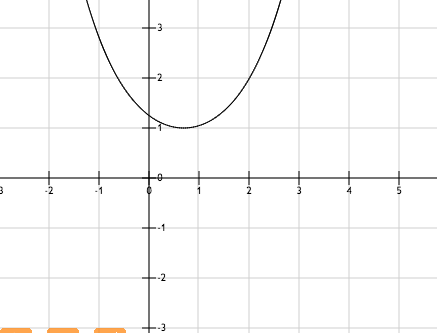
\includegraphics[scale=0.7]{prob1.png}

When \(t=ln2\) \(y=1\)


\end{homeworkProblem}

\begin{homeworkProblem}
\[4y'' - y =0 \]
\[y=Ae^{1/2t}+Be^{-1/2t}\]
Plug in the IV, we get
\[ A=1+\beta\]
\[B=1-\beta \]

As \(t \to \infty \) \( y \to 0 \) 
So \[  \beta = -1 \]

\end{homeworkProblem}

\begin{homeworkProblem}
\[ y'_1=2t y'_2=-t^{-2} \]
Plug it in, it equals to 0, so it's the solution \\
Since \(wronskian(x^2,x^{-1}) \neq 0\)
It is all the solution
\end{homeworkProblem}

\begin{homeworkProblem}

Plug it in, we get y1,y2 equals to 0, so it's the solution \\
But \[y=c1+c2t^{1/2}\] is not the solution.

It doesn't contradict the theorem, because \(yy''+y'^2=0\) is not a linear equation.
\end{homeworkProblem}

\begin{homeworkProblem}
Since y1 is the solution (verified by plug it in)
y2 is also the solution (verified by plug it in)
and \(wronskian(y1,y2) \neq 0 \)
So it forms a fundamental set of solutions
\end{homeworkProblem}

\begin{homeworkProblem}
Since \( r= \pm 2i \) The equation should be 
\[ y=Acos(2t)+Bsin(2t) \]

Plug in the IV, we get \[ A=0 B=1/2 \]

So the solution is

\[
y=\frac{1}{2}sin(2t)
\]

And the plot is  \\
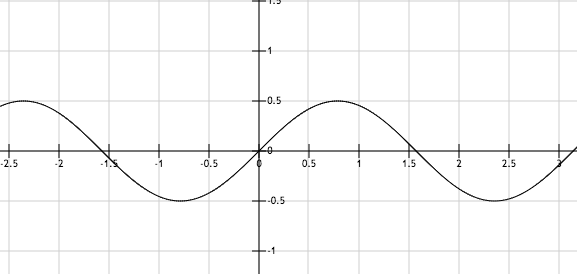
\includegraphics[scale=0.7]{prob2.png}

As \[t \to \infty y \to [-0.5,0.5] \]
\end{homeworkProblem}

\begin{homeworkProblem}
\[
r^2-\frac{1}{3}r+\frac{2}{3}=0
\]
Solve it, we get
\[
r=\frac{1\pm \sqrt{23}}{6}
\]

We plug it in with the initial value. We get 

\[
u(x) = -2/23 e^{x/6}*[\sqrt{23} sin((\sqrt{23} x)/6)-23 cos((\sqrt{23} x)/6)]
\]

2. plug in u=10, we get \( t= 10.76 \)
\end{homeworkProblem}

\begin{homeworkProblem}
1.We could get
\[
	r=\frac{3}{2}
\]
Plug it in with IV. We get
\[
y(t) =  e^{\frac{-3t}{2}}-\frac{5}{2}  e^{\frac{-3t}{2}} 
\]

2.plug in, we get \( t=\frac{2}{5} \) \\
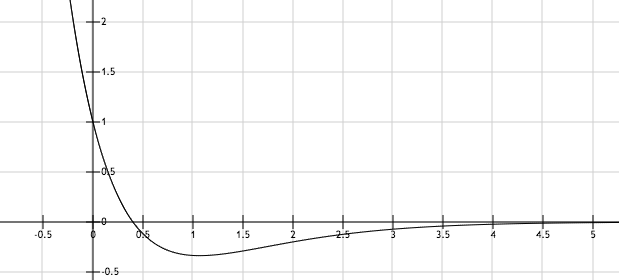
\includegraphics[scale=0.7]{prob3.png}

3.Let y'=0, we get
\[ 
y = \frac{-5}{3 e^{8/5}} \ at \ x = \frac{16}{15} \]

4.We plug in with the new IV. We get
\[
y(t) =  e^{\frac{-3t}{2}}-(b+\frac{3}{2})  e^{\frac{-3t}{2}} \]

When \( b=-\frac{3}{2} \) The solution will change
\end{homeworkProblem}

\begin{homeworkProblem}
\[
t^2y''+3ty'+y=0
\]
Let \( y_2=v(t)y_1 \)
\[
\begin{split}
y_2=vt^{-1} \\
y_2'=v't^{-1}-vt^{-2} \\
y_2''=v''t^{-1}-2v't^{-2}+2vt^{-3}\\
\end{split}
\]

Plug it in the old formula, we get

\[ tv''+v'=0 \]

Let \( r=v' \) Solve the formula above, we get

\[r=At^{-1} \]

We let A=1 so \[ r=t^{-1} \]

\[ v=ln(t) \]

So the solution will be 
\[
y=ln(t)t^{-1}\]
\end{homeworkProblem}

\end{document}
